\subsection{Celda Rauch (Deliyannis-Friend modificada)}

\subsubsection{Introducción}

Se busca mediante el uso de una celda de Rauch o también conocida como Deliyannis-Friend y la aproximación de Chebyshev para diseñar un filtro pasa banda con las siguientes parámetros:

\begin{table}[H]
    \centering
    \resizebox{0.5\textwidth}{!}{%
    \begin{tabular}{cc}
    \hline
    \multicolumn{2}{c}{Par\'ametros de diseño} \\ \hline
    Pendiente de pasabajos normalizado & -40dB/dec \\
    $f_p$ & 64KHz \\
    B & 1/10 \\
    $A_p$ & 3dB \\
    $Z_{in}(f)$ & $\geq 50K\Omega$ \\
    Filtro & Pasa-Banda\\\hline
    \end{tabular}%
    }
    \caption{Par\'ametros de diseño para el filtro a implementar}
    \label{ej22diseno}
\end{table}

Para ello debemos primero introducir la celda de Rauch que tiene la forma:

\begin{figure}[H]
    \centering
    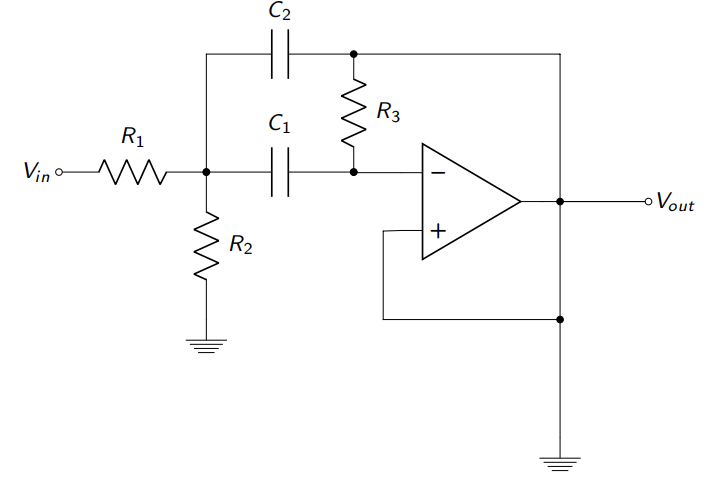
\includegraphics[scale = 0.6]{../Ejercicio2-DiseñoDeCeldas/2. CELDA RAUCH/Informe/circuito3.png}
    \caption{Celda de Rauch}
    \label{ej22cirbasic}
\end{figure}

Sin embargo, se observa que uno de los requisitos que debe cumplir el filtro es que $B = \frac{1}{Q} = \frac{1}{10}$, un valor de Q hace que las relaciones entre las resistencias R1 y R2 sean muy elevados, puesto que los valores de estas resistencias son inversa y directamente proporcionales, respectivamente, a este valor. Es por ello que se utiliza la versión modificada de la la celda Deliyannis-Friend que hace uso de un ciclo de realimentación positiva logrando asi valores elevados de Q.

\begin{figure}[H]
    \centering
    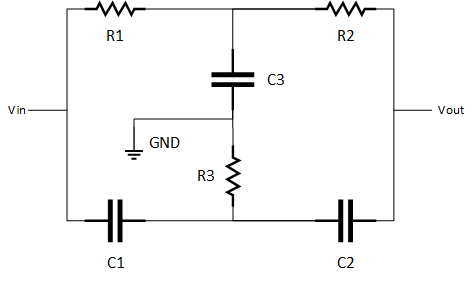
\includegraphics[scale = 0.6]{../Ejercicio2-DiseñoDeCeldas/2. CELDA RAUCH/Informe/circuito.png}
    \caption{Celda de Rauch Mejorada}
    \label{ej22cirbasic}
\end{figure}

Luego analizando el circuito con amplificadores operacionales ideales, o sea los $A_{vol} \longrightarrow \infty$, nos queda que la transferencia de la misma es:
\begin{equation}
    \label{ej22eqh}
    H(s) = \frac{sC2R2R3(RA+RB)}{s^2(C1C2R1R2R3RB) + s(C1R1R2RB + C2(R1R2RB - RA(R1R3 + R2R3))) + RB(R1+R2)}
\end{equation}
Conociendo que las resistencia de retroalimentación valen $RA = KR$ y $RB = (1-K)R$ y si conciderando los capacitores iguales ($C = C1 = C2$) obtenemos que:
\begin{equation}
    \label{ej22eqq}
    Q = \frac{\sqrt{R1R2R3(R1 + R2)}}{2R1R2 - \frac{K}{1 -K} (R1 + R2)R3}
\end{equation}
\begin{equation}
    \label{ej22eqw0}
    \omega_0^2 = \frac{R1+R2}{C^2R1R2R3}
\end{equation}
\begin{equation}
    \label{ej22eqg}
    G = \frac{R2R3}{2R1R2(K - 1) + KR3(R1 + R2)}
\end{equation}

\subsubsection{Dise\~no del Filtro con Chebyshev}

Para obtener una funci\'on trasferencia que cumpla con una plantilla, es posible utilizar la aproximación\'on de Chebyshev cuyas f\'ormulas caracter\'isticas se muestran en \ref{ej22eqche}.
\begin{equation}
    \begin{split}
        |H(s)|^2 = \frac{1}{1+\epsilon^2 \cdot T_n^2(\omega_N)}, \hspace{0.2cm} \epsilon = \sqrt{10^{\frac{A_p}{10}}-1}
    \end{split}
    \label{ej22eqche}
\end{equation}
Donde $T_n(\omega)$ son los polinomios de Chebyshev.

Debido a que se pide una pendiente de pasa bajos normalizado de $40dB/dec$, el orden de dicho pasa bajos es $n=2$, luego desnormalizando la aproximación, se encuentra que el orden del filtro pasa-banda es 4. En consecuencia, se
utilizarán 2 celdas Rauch de orden 2. Además, se pide una atenuación máxima en banda pasante de $3dB $ pero debido a las tolerancias de los componentes es óptimo una $A_p = 1dB$ para tener margen de error.

Luego, sabiendo que es un filtro pasa-banda podemos establecer la siguiente relación:
\begin{equation}
    \begin{split}
        f_0^2=f_P^+ \cdot f_P^-\\
        B=\frac{\Delta f}{f_0}\\
    \end{split}
    \label{ej22eqb}
\end{equation}

En resumen el filtro tendrá las siguientes propiedades:

\begin{table}[H]
    \centering
    \resizebox{0.4\textwidth}{!}{%
    \begin{tabular}{cc}
    \hline
    \multicolumn{2}{c}{Parámetros de diseño} \\ \hline
    Orden normalizado [n] & 2 \\
    Orden del filtro & 4 \\
    $f_p^+$ & 67kHz \\
    $f_p^-$ & 61kHz \\
    $A_p$ & 1dB \\ \hline
    \end{tabular}%
    }
    \caption{Propiedades del Filtro a Dise\~nar}
    \label{tab:TEMPLATE}
\end{table}

Teniendo en cuenta dichas propiedades, la transferencia del circuito sera:
\begin{equation}
\begin{split}
    H(s) &= \frac{s^2 B^2 \omega_0^2}{s^4+s^3 B \omega_0 1.0977343  + s^2 \omega_0^2 (2+B^2 1.1025103) + s B \omega_0^31.425625 + \omega_0^4}\\
     &= \frac{ 1.62 \cdot 10^9 s^2}{s^4+ 44.14 \cdot 10^3  s^3 +  3.25 \cdot 10^{11} s^2+  7.13 \cdot 10^{15} s+ 2.61 \cdot10^{22}}
\end{split}
\end{equation}

Como se menciono, utilizaremos dos celdas Rauch en cascada por lo que podemos diseñar el circuito separando la transferencia en dos etapas factorizando, resultando en:
\begin{equation}
    \label{ej22eqhf}
    H(s) = 1.62 \cdot 10^9\frac{s}{s^2 + 21.01\cdot 10^3 s + 1.47 \cdot 10^{11}}\frac{s}{s^2 + 23.13\cdot 10^3 s+ 1.77 \cdot 10^{11}}
\end{equation}

Por otro lado para asegurar que la impedancia de entrada nunca sea menor a $50k\Omega$, se utilizaron 4 amplificadores operacionales. Dos de ellas para el funcionamiento de las celdas, uno se coloco como un buffer entre las dos etapas, asegurando que no se altere ninguna etapa, y el cuarto fue utilizado como buffer de entrada, es decir impedancias muy altas a las frecuencias de interés.


\subsubsection{Selección de Componentes}

Conociendo entonces la función de transferencia del circuito dado en la ecuación \ref{ej22eqhf} es posible determinar los componentes indicados para el filtro deseado. Estos componentes lo podemos determinar utilizando las siguientes relaciones dado por Schaumann con $Q_0 = 1.5$, el factor óptimo de calidad de la celda Deliyannis-Friend sin mejora, y las respectivas $Q$ y $\omega_0$ del las etapas:

\begin{equation}
\begin{split}
    &Q = \frac{Q_0}{1-2\alpha Q_0^2} \hspace{1.5CM} \alpha = \frac{K}{1-K}\\
    &H_B = \frac{HQ}{Q_0(1-K)} \hspace{1CM}
    R3 = \frac{2Q_0}{\omega_0 C}\\
    &R' = \frac{R3}{4Q_0^2} \hspace{2.3CM}
    a = \frac{H}{2Q_0^2}\\
    &R1 = \frac{R'}{a} \hspace{2.3CM}
    R2 = \frac{R'}{1-a}
\end{split}
\label{ej22eqvalor}
\end{equation}

Despejando desde las ecuaciones \ref{ej22eqvalor} con $C = 1nF$ obtenemos los componentes a utilizar idealmente.

% Please add the following required packages to your document preamble:
% \usepackage{booktabs}
\begin{table}[H]
\centering
\begin{tabular}{@{}ccc@{}}
\toprule
\textbf{Componente}                     & \textbf{Primera Etapa} & \textbf{Segunda Etapa} \\ \midrule
\textbf{C {[}$nF${]}}                     & 1                      & 1                      \\
\textbf{R1 ${[}\Omega{]}$} & 30.11k                 & 27.63k                 \\
\textbf{R2 ${[}\Omega{]}$} & 895.25                 & 815.69                 \\
\textbf{R3 ${[}\Omega{]}$} & 7.82k                  & 7.13k                  \\
\textbf{RA ${[}\Omega{]}$} & 2.03k                  & 2.03k                  \\
\textbf{RB ${[}\Omega{]}$} & 9.97k                  & 9.97k                  \\ \bottomrule
\end{tabular}
\caption{Componentes Ideales}
\label{ej22tvalt}
\end{table}

\subsubsubsection{Sensibilidad de los Componentes}

Es importante conocer las sensibilidades de los parámetros previo a la selección de componentes, de esta manera tener una idea de que valores pueden variar sin causar grandes cambios en el circuito. 


% Please add the following required packages to your document preamble:
% \usepackage{booktabs}
\begin{table}[H]
\centering
\begin{tabular}{@{}cccc@{}}
\toprule
\textbf{Componentes} & $S_x^w$     & $S_x^H $                                    & $S_x^Q$                                                     \\ \midrule
\textbf{C}           & $-\frac{1}{2}$           & $-\frac{(K-1)R1R2+KR3(R1+R2) }{2R1R2(K-1)+KR3(R1+R2)}$   & $\frac{KR3(R1+R2)}{2(((K-1)2R2+KR3)R1+KR2R3)  }                       $\\
\textbf{R1}          & $-\frac{ R2 }{ 2(R1+R2)}$ & $-\frac{R1(2R2(K-1)+KR3)}{ 2R1R2(K-1)+KR3(R1+R2)}    $    & $-\frac{R2((2R1(K-1)-KR3)R2-KR1R3)}{2(R1+R2)((2R1(K-1)+KR3)R2+KR1R3)} $   \\
\textbf{R2}          & $-\frac{ R1}{2(R1+R2)} $ & $\frac{KR1R3 }{(2R2(K-1)+KR3)R1+KR2R3}  $                 &$-\frac{R1(((K-1)2R2-KR3)R1-KR2R3)}{2(R1+R2)(((K-1)2R2+KR3)R1+KR2R3)}   $ \\
\textbf{R3}          & $-\frac{1}{2}$            &$\frac{2R1R2(K-1)}{(2R2(K-1)+KR3)R1+KR2R3}$               &$\frac{R1((K-1)2R2-KR3)-KR2R3}{2(R1((K-1)2R2+KR3)+KR2R3) }  $            \\
\textbf{K}           &$0 $                &$-\frac{2KR1R2+KR3(R1+R2)}{2R1R2(K-1)+KR3(R1+R2)} $       & $\frac{KR3(R1+R2)}{ (K-1)(R1((K-1)2R2+KR3)+KR2R3)}                 $   \\ \bottomrule
\end{tabular}
\label{ej22tst}
\caption{Ecuaciones de Sensibilidad}
\end{table}

\subsubsubsection{Selección de Componentes a Utilizar}

Como los valores no suelen ser comerciales se debe adaptar los valores, luego teniendo en cuenta sus sensibilidades se selecciono los componentes a implementar como:

% Please add the following required packages to your document preamble:
% \usepackage{booktabs}
\begin{table}[H]
\centering
\begin{tabular}{@{}ccccc@{}}
\toprule
\textbf{Componente}                     & \textbf{Primera Etapa} & \textbf{Implementación} & \textbf{Segunda Etapa} & \textbf{Implementación} \\ \midrule
\textbf{C {[}nF{]}}                     & 1                      & 1                       & 1                      & 1                       \\
\textbf{R1 ${[}\Omega{]}$} & 30.11k                 & 27k+3k                  & 27.63k                 & 27k+560                 \\
\textbf{R2 ${[}\Omega{]}$} & 895.25                 & 560+330                 & 815.69                 & 560+150+100             \\
\textbf{R3 ${[}\Omega{]}$} & 7.82k                  & 4.7k+3k+100             & 7.13k                  & 6.2k+1k                 \\
\textbf{RA ${[}\Omega{]}$} & 2.03k                  & 2k                      & 2.03k                  & 2k                      \\
\textbf{RB ${[}\Omega{]}$} & 9.97k                  & 10k                     & 9.97k                  & 10k                     \\ \bottomrule
\end{tabular}
\label{ej22tvalr}
\caption{Valores de Componentes Seleccionados}
\end{table}

Luego, realizando un análisis de montecarlo con los componentes utilizados, resistencia de tolerancia $5\%$ y capacitor de tolerancia $20\%$, se obtuvo los posibles casos que enfrentaríamos en una medición experimental.

\begin{figure}[H]
    \centering
    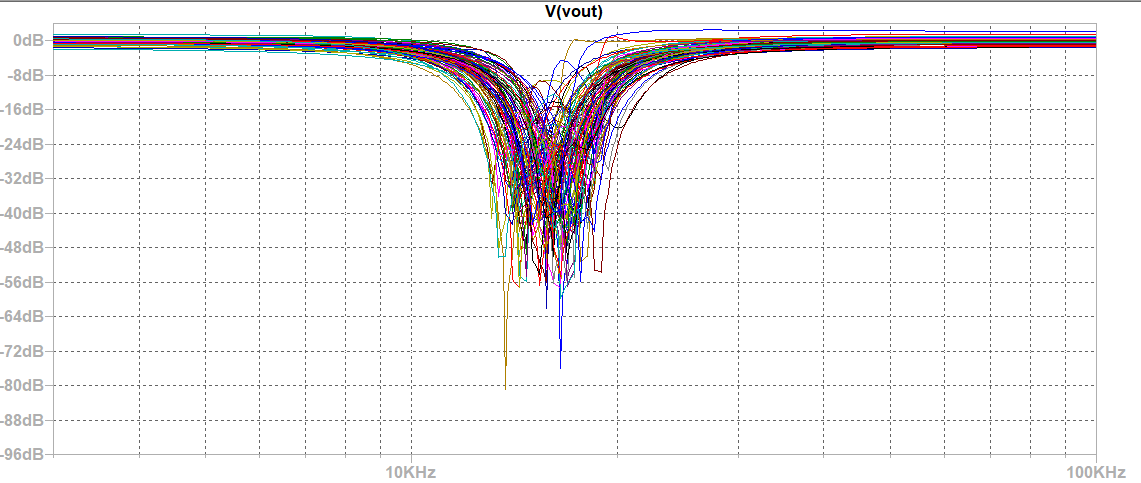
\includegraphics[scale = 0.65]{../Ejercicio2-DiseñoDeCeldas/2. CELDA RAUCH/Informe/monte.PNG}
    \caption{Análisis de Montecarlo}
    \label{ej22monteall}
\end{figure}

Para una representación mas gráfica se realizo un histograma de dispersión por etapa para la verificar del correcto uso de los componentes.

\begin{figure}[H]
    \centering
    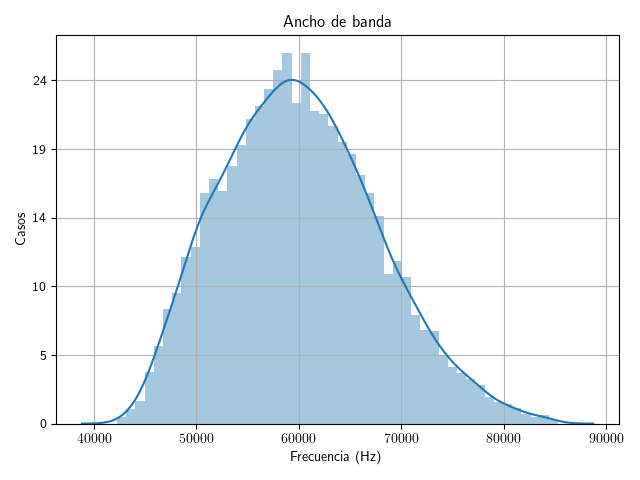
\includegraphics[scale = 0.5]{../Ejercicio2-DiseñoDeCeldas/2. CELDA RAUCH/Informe/disp1.png}
    \caption{Histograma de Dispersión de f0 de la Primera Etapa}
    \label{ej22dis1}
\end{figure}

\begin{figure}[H]
    \centering
    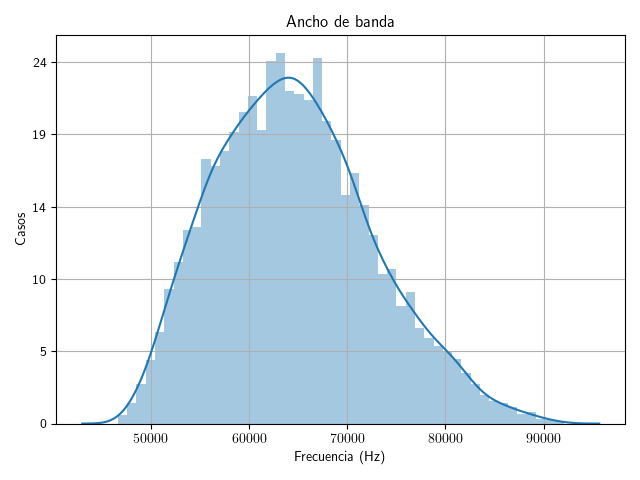
\includegraphics[scale = 0.5]{../Ejercicio2-DiseñoDeCeldas/2. CELDA RAUCH/Informe/disp2.png}
    \caption{Histograma de Dispersión de f0 de la Segunda Etapa}
    \label{ej22dis1}
\end{figure}


\subsubsection{Análisis de Experimental}

\subsubsubsection{Respuesta en Frecuencia}

Realizando un análisis en frecuencia, superponiendo resultados teóricos, simulados y experimental se obtuvo el siguiente gráfico:

\begin{figure}[H]
    \centering
    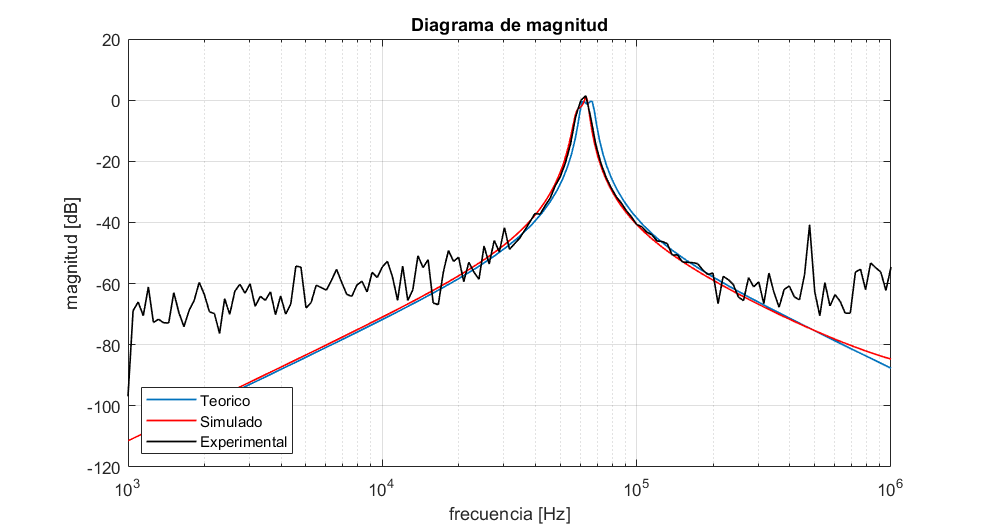
\includegraphics[scale = 0.6]{../Ejercicio2-DiseñoDeCeldas/2. CELDA RAUCH/Informe/bodemag.png}
    % \includegraphics[scale = 0.6]{bodepha.png}
    % \caption{Respuesta en Frecuencia del Circuito}
    % \label{ej22bode}
\end{figure}
\begin{figure}[H]
    \centering
    \includegraphics[scale = 0.6]{../Ejercicio2-DiseñoDeCeldas/2. CELDA RAUCH/Informe/bodepha.png}
    \caption{Respuesta en Frecuencia del Circuito}
    \label{ej22bode}
\end{figure}

En las frecuencias de interés, se puede observarse que se corresponden correctamente los valores medidos con los calculados, si bien con algunas leves diferencias debido a la tolerancia de los componentes pero se encuentra dentro de los resultados esperados. Es importante mencionar que como la atenuación a frecuencias lejanas al $f_0$, el circuito es susceptible al ruido, por lo que las mediciones se verán afectadas grandemente, creando oscilaciones indeseadas. Por otro lado, como se ve en la simulación y en la medición empírica, hay un salto de fase cuando $f>100kHz$, esta alteración es correspondiente al polo inducido por los amplificadores operacionales, dado que ahora no funcionan idealmente. 


\subsubsubsection{Impedancia de Entrada}

Como los amplificadores operacionales tienen una impedancia de entrada muy elevada, y no tener resistencias comparables para una correcta medición, se estudio la impedancia de entrada desde la simulación.

\begin{figure}[H]
    \centering
    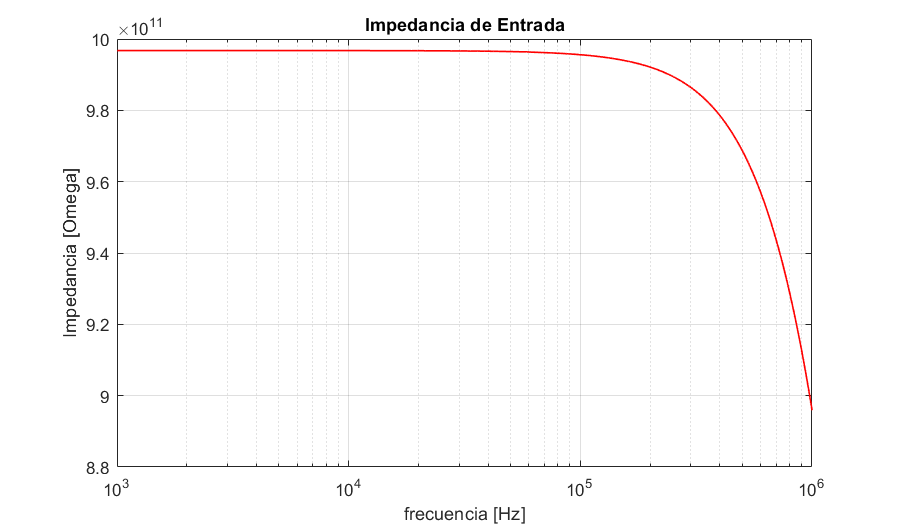
\includegraphics[scale = 0.5]{../Ejercicio2-DiseñoDeCeldas/2. CELDA RAUCH/Informe/zin.png}
    \caption{Impedancia de Entrada Simulado}
    \label{ej22zin}
\end{figure}

\subsubsubsection{Rango Dinámico}

Para el calculo de rango dinámico, se utiliza la ganancia máxima del circuito experimentado $G = 1.45dB = 1.18$. La tensi\'on m\'axima a la salida ser\'a 6V teniendo en cuenta que la alimentaci\'on $\pm 9V$. Por lo tanto, para hallar la m\'axima tensión sera:

\begin{equation}
    V_i^{MAX} = \frac{V_o^{MAX}}{1.8} = 5.08V
\end{equation}

Luego, suponiendo que la  tensi\'on m\'inima distinguible es el piso de ruido, ya que por debajo de este nivel de tensi\'on no es posible distinguir entre la se\~nal y el ruido, se considera entonces $V_o^{MIN}=10mV$, por lo que resulta que:

\begin{equation}
    V_i^{MIN} = 10mV
\end{equation}

Entonces obtenemos el rango dinámico como:

\begin{equation}
    RD = 20log(\frac{V_i^{MAX}}{V_i^{MIN}})= 54.12dB
\end{equation}

\subsubsection{Conclusión}

Si bien los resultados resultaron ser similares a la esperado, es indispensable mencionar que no es filtro preciso ya que los componentes utilizados fueron con tolerancias mayores a $5\%$ y no se utilizo prestes debido a la falta de un milímetro para conocer el valor utilizado. Por otro lado, se debe destacar la cualidad de esta celda de Rauch que se pudo obtener un elevado valor de factor de calidad debido a la realimentación positiva y negativa, pero se debe también tener cuidado ya que si los valores del ciclo de realimentación positiva no están bien diseñados, el circuito podría oscilar.
